\documentclass[11pt, a4paper]{article}

\usepackage{graphicx}
\usepackage[english]{babel}
\usepackage[utf8x]{inputenc}
\usepackage{amsmath}
\usepackage[a4paper,top=3cm,bottom=2cm,left=2cm,right=2cm,marginparwidth=1.75cm]{geometry}
\usepackage{amssymb}
\usepackage{subfig}

\graphicspath{ {./images} }

\makeatletter
\renewcommand*\env@matrix[1][*\c@MaxMatrixCols c]{%
  \hskip -\arraycolsep
  \let\@ifnextchar\new@ifnextchar
  \array{#1}}
\makeatother

\begin{document}

\setcounter{section}{9}
\section{Lecture 10: Kinematics of rigid bodies in 2D (16/03/2020)}
\subsection{Important side note}
From this point forward only radians will be used and never degrees. The usage of radians offers many advantages that degrees do not have such as simplifying math and being easier to work with in general. An example of this are the following equation that only apply when $\theta$ is in radians.
\begin{gather*}
    r\theta = s\\
    r\dot{\theta} = v_t\\
    r\ddot{\theta} = a_t\\
\end{gather*}

\begin{figure}[h]
  \centering
  \subfloat[Distance travelled]{{\includegraphics[width=40mm]{images/distance.png}}}%
  \qquad \qquad \qquad
  \subfloat[Tangential velocity]{{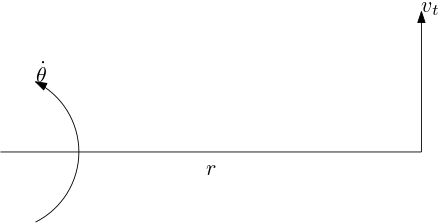
\includegraphics[width=40mm]{images/tangential_velocity.png}}}%
  \caption{Visualisation of the advantages of radians versus degrees for distance travelled and velocity}
\end{figure}

\subsection{Translations of a rigid body on a 2D plane}
There are 3 types of motion that can occur on a 2D plane. These are the exact same type motions that a given point mass can have and are as follows:
\begin{enumerate}
    \item Translation, or linear motion
    \item Rotations
    \item General motions on a plane
\end{enumerate}

\begin{figure}[h]
    \centerline{\includegraphics[width=80mm]{images/distance_vectors.png}}
    \caption{A random translation of a rigid body on a 2D plane}
\end{figure}
Geometric properties of vectors in 2D tell us that:
\begin{equation}
    \vec{r}_{B/A} = \vec{r}_B - \vec{r}_A
\end{equation}
Taking the time derivative of equation (1) gives the following:
\begin{equation}
    \frac{d\vec{r}_{B/A}}{dt} = \vec{v}_B - \vec{v}_A \qquad \text{or} \qquad \vec{v}_B = \vec{v}_A + \frac{d\vec{r}_{B/A}}{dt}
\end{equation}
$\vec{v}_B$ and $\vec{v}_A$ are absolute velocities since these are determine relative to the non-inertial $x,y$-coordinate system. Since $|\vec{r}_{B/A}| = c$, where $c$ is any random constant. From this we can conclude that the term $\frac{d\vec{r}_{B/A}}{dt} = 0$ since the derivative of a constant will always be 0. This concept holds because by the definition of a rigid body the distance between any random 2 point masses anywhere on the body will always be the same no matter the motion. This leaves us with the following equations:
\begin{gather}
    \vec{v}_B = \vec{v}_A\\
    \vec{a}_B = \vec{a}_A
\end{gather}
This effectively means that the acceleration and velocity of any point mass on a rigid body will always be the same no matter what.

\subsection{Rotations of a rigid body on a 2D plane}
All of the concept which apply to translation of a rigid body also still apply when analyzing the kinematics of a rotation. This leaves us with:
\begin{gather}
    \vec{\omega} = \frac{d\vec{\theta}}{dt}\\
    \vec{\alpha} = \frac{d\vec{\omega}}{dt} = \frac{d^2\vec{\theta}}{dt^2}\\
    \vec{\alpha}\,d\vec{\theta} = \vec{\omega}\,d\vec{\omega}
\end{gather}

From geometric properties of vectors that will not be derived here \footnote{Look at Hibbeler Dynamics book chapter 16.3 for more information}  the following relations arise:
\begin{gather}
    v = \omega r \Rightarrow \vec{v} = \vec{\omega} \times \vec{r}\\
    a_t = \alpha r \,,\, a_n = \omega^2 r \Rightarrow \vec{a} = \vec{a}_t + \vec{a}_n = \vec{\alpha} \times \vec{r} - \omega^2\vec{r}
\end{gather}

\subsection{Analyses of absolute motion}
Whenever a rigid body is making a general motion in a 2D plane there are usually several translations and rotations happening at the same time. Since Newton's law of motion $F =ma$ requires the motion to be absolute (I.E. a non-inertial frame of reference) we will need to express all motions relative to the same coordinate system. This can either be in polar coordinates $(r, \theta)$ or regular Cartesian coordinates $(x, y)$. The physics does not change and doesn't care how we choose to express a given motion but sometimes opting for a certain coordinate convention may simplify the mathematics a bit. An example of the general motion of a bar mechanism will be covered below.

\begin{figure}[h]
    \centerline{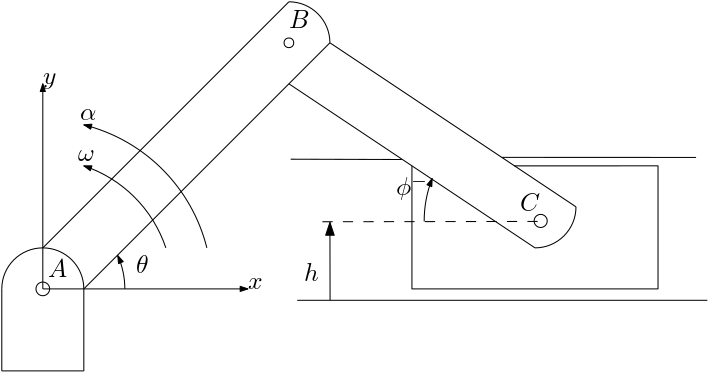
\includegraphics[width=75mm]{images/Bar_mechanism.png}}
    \caption{The bar mechanism for which the motion will be expressed}
\end{figure}

\begin{gather}
    x_B = L_1\cos(\theta)\\
    \dot{x}_B = -L_1\sin(\theta) \cdot \dot{\theta}\\
    \ddot{x}_B = -L_1\sin(\theta) \cdot \ddot{\theta} - L_1\sin(\theta) \cdot \dot{\theta}^2
\end{gather}
\begin{gather}
    x_C = L_1\cos(\theta) + L_2\cos(\phi)\\
    \dot{x}_C = -L_1\sin(\theta)\cdot \dot{\theta} - L_2\sin(\phi) \cdot \dot{\phi}\\
    \ddot{x}_C = -L_1\cos(\theta)\cdot \dot{\theta}^2 - L_1\sin(\theta) \cdot \ddot{\theta} - L_2\cos(\phi) \cdot \dot{\phi}^2 - L_2\sin(\phi)\cdot \ddot{\phi}\\
\end{gather}
\begin{gather}
    y_B = L_1\sin(\theta)\\
    \dot{y}_B = L_1\cos(\theta) \cdot \dot{\theta}\\
    \ddot{y}_B = -L_1\sin(\theta) \cdot \dot{\theta}^2 + L_2\cos(\theta)\cdot \ddot{\theta}
\end{gather}
\begin{gather}
    y_c = L_1\sin(\theta) - L_2\sin(\theta) = (L_1 - L_2)\sin(\theta)\\
    \dot{y}_C = (L_1 - L_2)\cos(\theta) \cdot \dot{\theta}\\
    \ddot{y}_C = -(L_1 - L_2)\sin(\theta) \cdot \dot{\theta}^2 + (L_1 - L_2)\cos(\theta) \cdot \ddot{\theta}
\end{gather}
From this we can see that the absolute acceleration of the joints in the object are described by equation (12), (16), (19) and (22) in terms of $\ddot{x}_B$, $\ddot{x}_C$ ,$\ddot{y}_B$ and $\ddot{y}_C$. These are the equations that would be relevant for Newton's law $F = ma$.
\end{document}
